\subsection{Применение системы компьютерного зрения в антропометрии для пошива одежды (E-Tailor)}
Программа <<E-Taloir>> предназначена для пошива одежды.
При запуске программы появляется главное окно формы \ref{img42}

\begin{itemize}
\item <<Measure Me>> В рабочей области отображается видеопоследовательность, область обнаружения объектов и извлечение антропометрических признаков;
\item <<Credit>> Контакты с командой разработчиков;
\item <<Exit>> Позволяет осуществить выход из программы.
\end{itemize}

\begin{figure}[ht!]
\centering
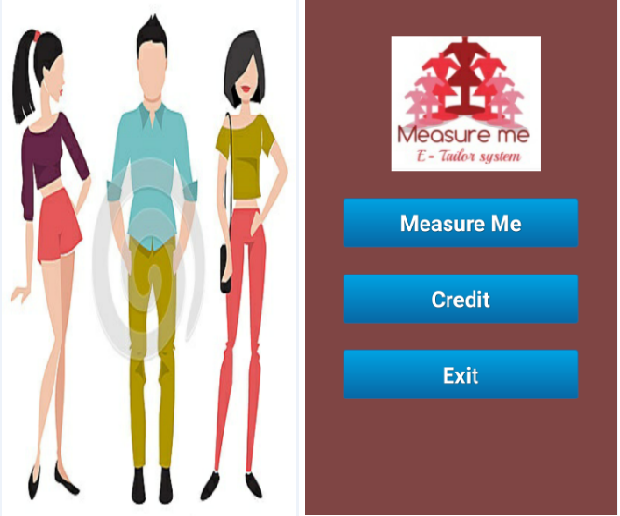
\includegraphics [scale=0.5] {images/h42.png}
\begin{center}
%\captionsetup{justification=justified, labelsep=period}
\caption{Основный интерфейс приложения E-Tailor} \label{img42}
\end{center}
\end{figure}
\textbf{Основные функции приложения E-Tailor \ref{img43}}

\begin{itemize}
	\item Позволять пользователям добавлять информацию;
	\item Показать 3D-модель на основе антропометрических признаков и классификации данных;
	\item Позволять пользователям выбрать марки одежды и классифицировать размеры одежды.
\end{itemize}

\begin{figure}[ht!]
\centering
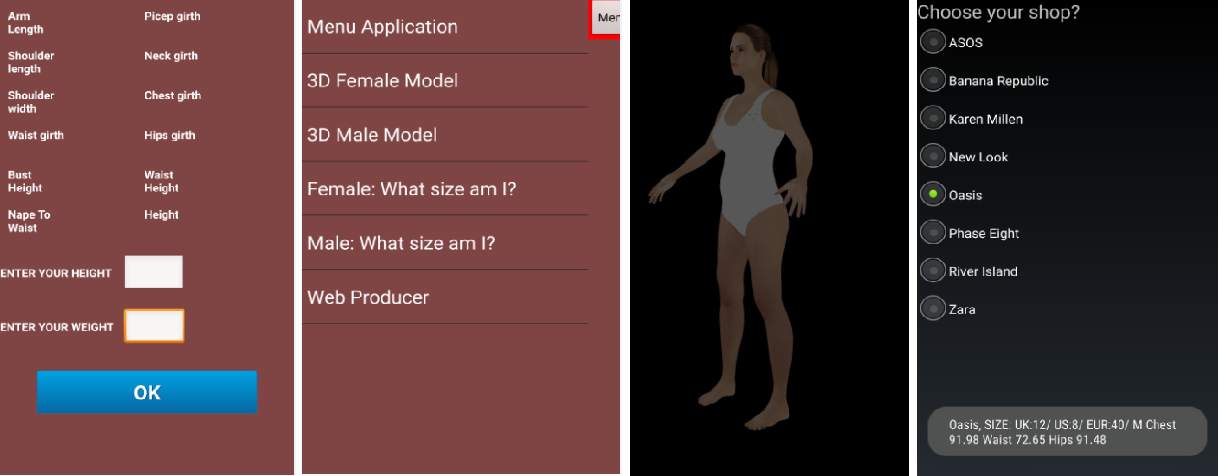
\includegraphics [scale=0.5] {images/h43.png}
\begin{center}
%\captionsetup{justification=justified, labelsep=period}
\caption{Результат функции выбора размеров одежды} \label{img43}
\end{center}
\end{figure}

